\section{Motor BLDC}
\label{sec:motor_bldc}

Para fins de resultados pertinentes à equipe Albatroz Aerodesign, designou-se o motor \textit{Scorpion A-5025-310Kv} como unidade sob ensaio. A caracterização do motor exige a identificação experimental de seus parâmetros elétricos e mecânicos, os quais alimentam tanto o modelo dinâmico quanto o observador de estados.

\subsection{Parâmetros Elétricos}
\label{sec:params_eletricos}

Para a determinação da resistência e da indutância de fase, emprega-se o ensaio de rotor bloqueado, cujo circuito equivalente está ilustrado na Figura \ref{fig:circuito_estrela_bldc}. O travamento mecânico do eixo impede a indução de forças contraeletromotrizes decorrentes de micro-oscilações, reduzindo o modelo elétrico do motor a uma malha puramente passiva em ligação estrela\footnote{Este equacionamento é válido independentemente do fechamento interno real da máquina. Para um motor fechado em delta, a impedância medida linha a linha equivale a duas fases em série em paralelo com a terceira ($Z_{linha} = \frac{2}{3}Z_{\Delta}$). Como a transformação para o modelo equivalente em estrela requer $Z_Y = \frac{Z_{\Delta}}{3}$, chega-se à mesma relação final $Z_Y = \frac{Z_{linha}}{2}$, permitindo modelar o motor a partir dos terminais como uma caixa preta.}.

\begin{figure}[H]
    \centering
    \caption{Circuito Equivalente do Motor BLDC (Rotor Bloqueado) }

    \begin{tikzpicture}[transform shape, american]
        % Ponto Neutro
        \node[circ] (N) at (0,0) {};
        \node[above left, xshift=-0.1cm] at (N) {$N$};

        % Fase U (Para Cima)
        \draw (N) to[american resistor, l=$R_{fase}$] (0,2)
                  to[cute inductor, l=$L_{fase}$] (0,4)
                  node[ocirc] (U) {}
                  node[above] {Fase $U$};

        % Fase V (Para a Direita/Baixo) - Ângulo de -30°
        \draw (N) to[american resistor, l=$R_{fase}$] (1.732,-1)
                  to[cute inductor, l=$L_{fase}$] (3.464,-2)
                  node[ocirc] (V) {}
                  node[right] {Fase $V$};

        % Fase W (Para a Esquerda/Baixo) - Ângulo de 210°
        \draw (N) to[american resistor, l_=$R_{fase}$] (-1.732,-1)
                  to[cute inductor, l_=$L_{fase}$] (-3.464,-2)
                  node[ocirc] (W) {}
                  node[left] {Fase $W$};

        % --- Indicação do Ensaio (Medição Linha a Linha) ---

        % Linhas de chamada (tracejadas) saindo de U e V para a direita
        \draw[dashed, blue!70!black] (U) -- (5.5, 4);
        \draw[dashed, blue!70!black] (V) -- (5.5, -2);

        % Seta dupla indicando a medição com texto explicativo
        \draw[<->, blue!70!black, thick] (5.5, 3.9) -- node[fill=white, align=center, text=black] {Ensaio Linha a Linha \\ $V_{DC}, I_{DC}$ (Resistência) \\ $L_{linha}$ (Indutância) \\ \small \textit{Equivalente a 2 em série}} (5.5, -1.9);

        % Marcação do caminho da corrente para ficar mais didático (Opcional)
        \draw[->, red, thick, rounded corners=5mm] (0.5, 3.5) -- (0.5, 0.5) -- (3.0, -1.0) node[pos=0.8, above right] {$I_{ensaio}$};

    \end{tikzpicture}
    \label{fig:circuito_estrela_bldc}

    \small Fonte: Autor (2026)
\end{figure}

A resistência de fase é medida aplicando-se uma corrente contínua entre dois terminais do motor. Nesta condição, a reatância indutiva é nula e a queda de tensão ocorre integralmente sobre as resistências. Medindo-se a tensão ($V_{DC}$) e a corrente ($I_{DC}$), a resistência de fase equivalente é calculada por:

\begin{equation}
    R_{fase} = \frac{V_{DC}}{2\,I_{DC}}
    \label{eq:resistencia_fase}
\end{equation}


De maneira análoga, com o rotor ainda imobilizado, conduz-se o ensaio para a
obtenção da indutância de fase através do método da ressonância. Motores BLDC
aplicados em aeromodelismo, como o \textit{Scorpion A-5025}, geralmente possuem
ímãs montados na superfície do rotor (SPM, \textit{Surface Permanent
Magnet}). O entreferro efetivamente uniforme característico dessa topologia
torna a saliência magnética insignificante, permitindo assumir que as
indutâncias de eixo direto ($L_d$) e em quadratura ($L_q$) são aproximadamente
iguais ($L_d \approx L_q \approx L_s$), onde $L_s$ é a indutância síncrona da
máquina \cite{Krishnan2017}.

Na ausência de um medidor LCR, o ensaio consiste em associar um capacitor de
valor conhecido ($C$) em paralelo com o enrolamento da máquina, formando um
circuito ressonante $LC$ alimentado por uma fonte senoidal de frequência
variável através de um resistor série $R$, conforme a
Figura~\ref{fig:circuito_ressonancia_v2}. Ao varrer a frequência da fonte até
atingir a frequência de ressonância ($f_r$), na qual a impedância do tanque
$LC$ é máxima e a tensão sobre ele atinge seu valor de pico, a indutância pode
ser estimada \cite{Fitzgerald2014}. A condição de ressonância corresponde ao
ponto em que a reatância do circuito se anula, restando apenas as componentes
resistivas. Após determinar a indutância equivalente medida entre dois
terminais ($L_{linha}$), a indutância de fase individual é obtida pela relação
de ressonância:

\begin{figure}[htbp]
    \centering
    \caption{Circuito de ensaio de ressonância: resistor $R$ em série com o
    paralelo $L$--$C$, com a tensão de ressonância medida sobre o tanque.}
    \label{fig:circuito_ressonancia_v2}
    \begin{circuitikz}[american, scale=1.1, transform shape]
        % ---- Fonte e resistor série (ramo superior) ----
        \draw (0,0) to[sV, l=$v_{in}$] (0,3);
        \draw (0,3) to[R, l=$R$, i>^=$i_{in}$] (3,3);
        % ---- Nó de medição (saída do gerador / topo do tanque) ----
        \node[circ] (A) at (3,3) {};
        \node[anchor=south] at (3,3.2) {\footnotesize nó A};
        % ---- Ramo do indutor ----
        \draw (A) to[L, l=$L_{fase}$] (3,0);
        % ---- Ramo do capacitor (em paralelo) ----
        \draw (A) -- (5.5,3);
        \draw (5.5,3) to[C, l=$C$] (5.5,0);
        % ---- Trilho de terra (retorno) ----
        \draw (0,0) -- (5.5,0);
        \node[circ] (G) at (3,0) {};
        \node[ground] at (1.5,0) {};
    \end{circuitikz}

    \fonte{Autor (2026).}
\end{figure}

\begin{equation}
    f_r = \frac{1}{2\pi\sqrt{L_{linha} \cdot C}}
    \implies
    L_{linha} = \frac{1}{C\,(2\pi f_r)^2}
    \label{eq:ressonancia_L}
\end{equation}

Considerando a topologia de conexão dos enrolamentos, a indutância de fase
individual é dada por:

\begin{equation}
    L_{fase} = \frac{L_{linha}}{2}
    \label{eq:indutancia_fase}
\end{equation}

Como os laboratórios disponíveis não contam com medidor LCR, essa medição
isolada pode carregar erros consideráveis. Por isso a indutância também é
estimada por um segundo método, a partir dos registros de tensão e corrente de
fase feitos com o motor girando (\autoref{sec:resultado_setup_scope}).

O método usa o circuito fasorial de uma fase para cada harmônico
(\autoref{sec:analise_harmonica}, \autoref{fig:circuito_ajuste_L}), válido
com o motor em regime, sem saturação e com parâmetros constantes na faixa de
frequências analisada. Isolando a impedância do enrolamento na
\autoref{eq:Lajuste_passo5}:

\begin{equation}
    R_s + jX_{L,h} = \frac{\dot{V}_h - \dot{E}_h}{\dot{I}_h}
    \quad\Longrightarrow\quad
    L_s = \frac{1}{h\,\omega_e}\,
    \mathrm{Im}\!\left\{\frac{\dot{V}_h - \dot{E}_h}{\dot{I}_h}\right\}
    \label{eq:Lajuste_passo6}
\end{equation}

\noindent Os fasores $\dot{V}_h$ e $\dot{I}_h$ são obtidos pela transformada
de Fourier dos registros de tensão e corrente de fase. O fasor $\dot{E}_h$
vem da constante $K_e$, medida a vazio, e da rotação, com a fase ajustada ao
registro. A \autoref{eq:Lajuste_passo6} usa só a parte imaginária, de modo que
$L_s$ não depende de $R_s$; a parte real fornece uma verificação de $R_s$.

Na prática, cada harmônico e cada registro fornecem uma estimativa de $L_s$
afetada por ruído. As estimativas são combinadas por mínimos quadrados: escolhe-se
o $L_s$ que minimiza a diferença entre a corrente medida e a prevista pela
\autoref{eq:Lajuste_passo5},

\begin{equation}
    L_s = \arg\min_{L} \sum_{h \geq 1} \left|\dot{I}_h -
    \frac{\dot{V}_h - \dot{E}_h}{R_s + jh\omega_e L}\right|^2
    \label{eq:ajuste_L_harm}
\end{equation}

\noindent o que dá naturalmente mais peso aos harmônicos de maior amplitude, em especial à
fundamental, onde o ruído pesa menos e a hipótese (iii) é mais confiável. O
procedimento é repetido para registros em várias rotações e com os dois
controladores, e o resultado é comparado ao da ressonância pelo erro com que
cada valor prevê a corrente.

\subsection{Parâmetros Mecânicos}
\label{sec:params_mecanicos}

A dinâmica mecânica do motor é governada pela equação de balanço de torques no eixo rotativo, como visto na \autoref{eq:bldc_mecanica}.

Os ensaios de atrito e de inércia descritos nesta subseção foram conduzidos
sem a hélice acoplada ao eixo, de modo que $B$, $\tau_c$ e $J$ correspondem
exclusivamente ao conjunto girante do próprio motor (rotor, eixo e
rolamentos). Com a hélice montada para os ensaios aerodinâmicos
(\autoref{sec:coef_aero_bancada}), o diâmetro do modelo utilizado
entra como $D_{prop}$ na \autoref{eq:Prop_coeff1}, conforme a nomenclatura $D \times P$ da
\autoref{sec:helice_aerodinamica}.

Para a caracterização experimental, o motor BLDC é acionado por um Controlador Eletrônico de Velocidade (ESC) comercial. O torque eletromagnético ($T_e$) é proporcional à corrente de eixo em quadratura ($I_q$), e os ensaios foram conduzidos com as correntes e tensões de fase adquiridas diretamente por osciloscópio. O esquema de aquisição e as formas de onda resultantes estão ilustrados na Figura~\ref{fig:circuito_esc_correntes}.

\begin{figure}[H]
    \centering
    \caption{Esquema de Medição com ESC e Transformação de Correntes ($abc \to dq$)}

    % --- PARTE 1: CIRCUITO DE \textit{hardware} COM AJUSTES DE LEGENDA ---
    \begin{tikzpicture}[auto, node distance=2cm, >=latex']

        % --- Blocos principais ---
        \node [draw, rectangle, minimum height=3em, minimum width=4em] (bat) {Bateria};

        % Aumentei para 8em para comportar o deslocamento das fases com folga
        \node [draw, rectangle, minimum height=8em, minimum width=4em, right=of bat, node distance=2.5cm] (esc) {ESC};

        % BLDC posicionado à direita
        \node [draw, rectangle, rounded corners=8pt, minimum height=8em, minimum width=5em, right=of esc, node distance=6.5cm] (motor) {BLDC};

        % DAQ centralizado abaixo
        \node [draw, rectangle, minimum height=4em, minimum width=10em, below=of esc, node distance=4.5cm, xshift=3.25cm] (daq) {Osciloscópio};

        % --- Conexões Bateria -> ESC ---
        \draw [thick] ([yshift=0.3cm]bat.east) -- node[above] {$V_{DC}$} ([yshift=0.3cm]esc.west);
        \draw [thick] ([yshift=-0.3cm]bat.east) -- node[below] {GND} ([yshift=-0.3cm]esc.west);

        % --- Coordenadas das Fases (A, B, C) ---
        % Deslocadas para cima (+0.5cm) para não bater no centro (0) do Eixo
        \coordinate (esc_a) at ([yshift=1.5cm]esc.east);
        \coordinate (esc_b) at ([yshift=0.5cm]esc.east);
        \coordinate (esc_c) at ([yshift=-0.5cm]esc.east);

        \coordinate (mot_a) at ([yshift=1.5cm]motor.west);
        \coordinate (mot_b) at ([yshift=0.5cm]motor.west);
        \coordinate (mot_c) at ([yshift=-0.5cm]motor.west);

        % --- Conexões das Fases ---
        \draw [thick] (esc_a) -- node[above, pos=0.5, font=\large\bfseries] {A} (mot_a);
        \draw [thick] (esc_b) -- node[above, pos=0.5, font=\large\bfseries] {B} (mot_b);
        \draw [thick] (esc_c) -- node[below, pos=0.5, font=\large\bfseries] {C} (mot_c);

        % --- Sensores de Corrente (Intercalados) ---
        % Sensor A (Violeta) próximo ao ESC
        \node [draw, circle, minimum size=0.45cm, inner sep=0pt, thick, fill=white] (sensA) at ([xshift=1.2cm]esc_a) {};
        % Sensor B (Teal) próximo ao Motor
        \node [draw, circle, minimum size=0.45cm, inner sep=0pt, thick, fill=white] (sensB) at ([xshift=1.5cm]esc_b) {};

        % --- Sensor de Posição Óptico (No Eixo Central) ---
        \node [draw, rectangle, minimum height=2em, right=of motor, node distance=2.2cm] (enc) {Sensor};
        % O Eixo sai do centro exato (0), onde agora não há fios
        \draw [thick, dashed] (motor.east) -- node[above] {Eixo} (enc.west);

        % --- Conexões de Dados para o SAME (Intercaladas) ---
        % Sensor A desce mais (3.5cm)
        \draw [->, dashed, violet, thick] (sensA.south) -- ++(0,-3.5) -| ([xshift=-1.2cm]daq.north);

        % Sensor B desce menos (1.8cm)
        \draw [->, dashed, teal, thick] (sensB.south) -- ++(0,-3.5) -| ([xshift=-0.9cm]daq.north);

        % Sensor de posição vem pela lateral
        \draw [->, dashed, thick] (enc.south) |- (daq.east) node[pos=0.8, above] {$\theta, \omega$};

        % --- Label de transformação ---
        \node [below, font=\scriptsize, text width=5cm, align=center] at (daq.south) { $I_c = -(I_a + I_b)$ \\ Clarke \& Park $\to I_d, I_q$};

    \end{tikzpicture}

    \vspace{0.8cm} % Espaço entre o circuito e os gráficos

    % --- PARTE 2: GRÁFICOS DAS CORRENTES COM AJUSTES DE EIXO ---
    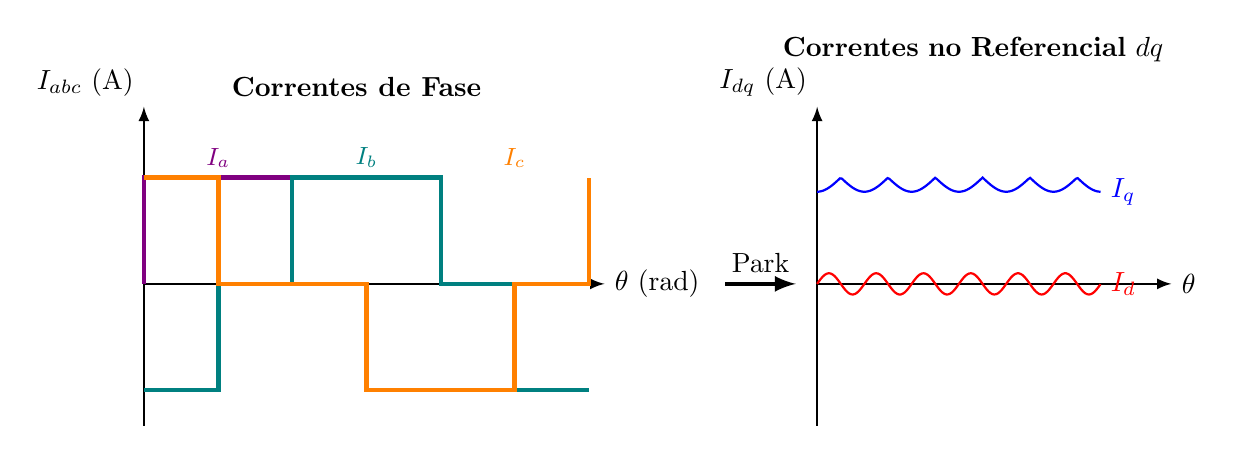
\begin{tikzpicture}[scale=0.9, >=latex]

        \begin{scope}[xshift=0cm]
            \draw[->, thick] (0,-2) -- (0,2.5) node[above left] {$I_{abc}$ (A)};
            \draw[->, thick] (0,0) -- (6.5,0) node[right] {$\theta$ (rad)};

            % Curva Ia (120 graus ligada, 60 desligada)
            \draw[ultra thick, violet] (0,0) -- (0,1.5) -- (2.09,1.5) -- (2.09,0) -- (3.14,0) -- (3.14,-1.5) -- (5.23,-1.5) -- (5.23,0) -- (6.28,0);
            \node[above, violet, font=\small\bfseries] at (1.05, 1.5) {$I_a$};

            % Curva Ib (Atrasada 120 graus)
            \draw[ultra thick, teal] (0,-1.5) -- (1.05,-1.5) -- (1.05,0) -- (2.09,0) -- (2.09,1.5) -- (4.19,1.5) -- (4.19,0) -- (5.23,0) -- (5.23,-1.5) -- (6.28,-1.5);
            \node[above, teal, font=\small\bfseries] at (3.14, 1.5) {$I_b$};

            % Curva Ic (Adiantada 120 graus)
            \draw[ultra thick, orange] (0,1.5) -- (1.05,1.5) -- (1.05,0) -- (3.14,0) -- (3.14,-1.5) -- (5.23,-1.5) -- (5.23,0) -- (6.28,0) -- (6.28,1.5);
            \node[above, orange, font=\small\bfseries] at (5.23, 1.5) {$I_c$};

            \node[above] at (3, 2.5) {\textbf{Correntes de Fase}};
        \end{scope}

        % --- Seta de Transformação ---
        \draw[->, ultra thick] (8.2, 0) -- node[above, black] {Park} (9.2, 0);

        % --- Gráfico 2: Correntes FOC (dq) com RIPPLE ---
        \begin{scope}[xshift=9.5cm]
            \draw[->, thick] (0,-2) -- (0,2.5) node[above left] {$I_{dq}$ (A)};
            \draw[->, thick] (0,0) -- (5,0) node[right] {$\theta$};

            % Curva Iq (Com ripple de comutação - 6 pulsos)
            \draw[thick, blue, domain=0:4, samples=150] plot (\x, {1.5 - 0.2*abs(cos(4.71*\x r))}) node[right] {$I_q$};

            % Curva Id (Oscilando em torno de zero)
            \draw[thick, red, domain=0:4, samples=150] plot (\x, {0.15*sin(9.42*\x r)}) node[right] {$I_d$};

            \node[above, text width=5cm, align=center] at (2.2, 3) {\textbf{Correntes no Referencial $dq$}};
        \end{scope}

    \end{tikzpicture}

    \label{fig:circuito_esc_correntes}
    \small Fonte: Autor (2026)
\end{figure}

Registram-se as correntes de pelo menos duas fases (ex.: $I_a$ e $I_b$); a terceira é reconstruída por $I_c = -(I_a + I_b)$, pois não há neutro acessível. Aplicam-se as transformadas de Clarke e Park para mapear as grandezas do referencial trifásico estacionário ($abc$) para o referencial síncrono girante ($dq$)\footnote{Devido à comutação trapezoidal (6-\textit{step}) do ESC, as correntes apresentam harmônicos que produzem \textit{ripple} nas componentes $I_d$ e $I_q$ após a transformada de Park. Utiliza-se o valor médio filtrado de $I_q$, representativo do torque eletromagnético médio em regime permanente.}.

Os ensaios de atrito e de inércia descritos a seguir foram conduzidos numa
montagem com osciloscópio de laboratório: o motor é acionado por um ESC
comercial, com a rotação do eixo medida por tacômetro óptico e as grandezas
elétricas de fase capturadas nos canais analógicos do osciloscópio.

\subsubsection{Coeficiente de Atrito Viscoso}
\label{sec:atrito_viscoso}

Para extrair os coeficientes de atrito ($B$ e $\tau_c$) \footnote{O parâmetro $\tau_c$ agrega atrito seco dos rolamentos e perdas por histerese no ferro do estator; a regressão linear não os separa.}, estabiliza-se a rotação do motor a vazio em múltiplos patamares. Em regime permanente ($\frac{d\omega_m}{dt} = 0$), o torque eletromagnético anula exatamente as perdas mecânicas:

\begin{equation}
    T_{e,k}= B\omega_{m,k} + \tau_c
    \label{eq:ensaio_vazio_iq}
\end{equation}

Os parâmetros $B$ e $\tau_c$ são obtidos através de uma regressão linear sobre os pontos experimentais médios $(\omega_{m,k}, T_{e,k})$ para cada patamar de rotação, o $\omega_{m,k}$ é medido através de um tacômetro digital para validação.

\subsection{Identificação do Coeficiente de Torque da Hélice em Bancada}
\label{sec:coef_aero_bancada}

São ensaiadas duas hélices APC, 15x6E e 17x10E. O objetivo é verificar a
bancada pela curva de torque, que o fabricante não fornece diretamente em forma
de coeficiente; a curva de tração fica para os ensaios da equipe. Com a hélice
montada no eixo e sem vento incidente ($J = 0$), o motor é levado por patamares
de rotação crescente, até no máximo \num{10000} RPM, seguindo o fluxo da
\autoref{fig:fluxo_ensaio_helice}. Em cada patamar, depois que a rotação
estabiliza, registram-se a rotação, o torque eletromagnético e a
densidade do ar, calculada pela lei dos gases ideais a partir da pressão
absoluta $P_{atm}$ e da temperatura absoluta $T$ do ambiente
\cite{Moran2018}, com $R_{ar} = \SI{287,05}{\joule\per\kilo\gram\per\kelvin}$:

\begin{equation}
    \rho = \frac{P_{atm}}{R_{ar}\,T}
    \label{eq:densidade_calculo}
\end{equation}

\begin{figure}[H]
    \centering
    \caption{Fluxo do ensaio de identificação do coeficiente de torque da hélice}
    \label{fig:fluxo_ensaio_helice}
    \begin{tikzpicture}[
        font=\small,
        box/.style={draw, rounded corners, align=center, minimum height=1cm, minimum width=3.1cm, text width=2.9cm},
        arrow/.style={-{Latex}, thick}
    ]
        \node[box] (duty)  at (0,0)   {Novo patamar\\de rotação};
        \node[box] (estab) at (3.6,0) {Aguarda\\estabilizar};
        \node[box] (reg)   at (7.2,0) {Registra rotação,\\torque e $\rho$};
        \node[box] (calc)  at (10.8,0){Calcula $C_Q$\\do patamar};

        \draw[arrow] (duty) -- (estab);
        \draw[arrow] (estab) -- (reg);
        \draw[arrow] (reg) -- (calc);
        \draw[arrow] (calc.south) -- ++(0,-0.45) -| node[pos=0.25, below, font=\scriptsize]{próximo patamar} (duty.south);
    \end{tikzpicture}

    Fonte: Autor (2026)
\end{figure}

O torque eletromagnético é calculado com as correntes de fase medidas,
projetadas no ângulo $\hat{\theta}$ estimado pelo observador:

\begin{equation}
    \hat{T}_e = \tfrac{3}{2}\,K_e\,p\,\big(f_\alpha(\hat{\theta})\,i_\alpha
               + f_\beta(\hat{\theta})\,i_\beta\big),
    \label{eq:torque_corrente_medida}
\end{equation}

\noindent em que $f_{\alpha\beta}$ é a forma normalizada da força
contraeletromotriz. O observador entra apenas com o ângulo e a velocidade; as
correntes são as medidas, e não as estimadas, porque o \textit{chattering} das
correntes estimadas não tem média nula e se acumularia na média do patamar,
em que o torque da hélice é muito menor que a ondulação do acionamento em seis
passos. Descontadas as perdas a vazio do motor,
$B\,\omega + \tau_c$, o coeficiente de cada patamar sai da
\autoref{eq:Prop_coeff1}. A referência são as tabelas de desempenho do
fabricante \cite{apc_performance_data} na condição $J = 0$, convertendo-se
$C_P$ para $C_Q$ pela \autoref{eq:cq_from_cp}. Como o coeficiente varia com a
rotação (efeito do número de Reynolds), ele é comparado por patamar, e não
como um valor único.

\subsection{Parametrização do SMO}
\label{sec:param_smo}

Com os parâmetros do motor obtidos, restam os ganhos do observador
($\Gamma_{s1}$, $\Gamma_{s2}$ e $\Gamma_t$). Ganhos elevados aceleram a
convergência, mas aumentam o ruído na força contraeletromotriz estimada, e o
polo do estimador atenua esse ruído ao custo de atraso. Como a frequência
elétrica varia ao longo da operação, o ajuste manual é laborioso e pouco
reprodutível, e por isso os ganhos são obtidos por otimização sobre a
simulação do conjunto motopropulsor (\autoref{sec:otimizacao_revbib}). Nesta
seção, as grandezas da planta simulada são chamadas de ``reais'', em
contraposição às estimadas pelo observador.

A função-custo mede o seguimento das grandezas que a bancada entrega, o torque
e a velocidade, e não grandezas internas do observador. A simulação percorre
um perfil de patamares de velocidade, e em cada patamar $q$ usa-se a segunda
metade, já em regime. Os resíduos de torque e de velocidade são avaliados pelo
RMSE (\autoref{eq:metricas_erro}), normalizado pelo desvio-padrão do sinal
real no patamar ($\sigma_q$):

\begin{equation}
    g_{T,q} = \frac{\mathrm{RMSE}\big(\hat{T}_{q} - T_{q}\big)}{\sigma_{T,q}},
    \qquad
    g_{\omega,q} = \frac{\mathrm{RMSE}\big(\hat{\omega}_{q} - \omega_{q}\big)}{\sigma_{\omega,q}}
    \label{eq:termos_seguimento}
\end{equation}

\noindent e o custo é a média ponderada sobre os $M$ patamares:

\begin{equation}
    J(\mathbf{x}) = \frac{1}{M}\sum_{q=1}^{M}
        \Big( w_T\,g_{T,q} + w_\omega\,g_{\omega,q}\Big),
    \qquad w_T = \num{1,0}, \quad w_\omega = \num{0,5}
    \label{eq:custo_autotuning}
\end{equation}

\noindent O peso maior no torque reflete o interesse da caracterização
propulsiva. O RMSE foi preferido à perda de Huber porque, com os resíduos
desta planta, o Huber comprimia o termo de torque e invertia na prática os
pesos (\autoref{sec:funcao_custo_revbib}). O valor de $J$ é um índice relativo
para orientar a busca, e não um erro percentual.

A otimização é feita sobre os ganhos $\Gamma = K\,T_s$
(\autoref{eq:discretizacao_coeff_smo}), que não dependem do passo de
amostragem; o \textit{firmware} recupera seus ganhos por $K = \Gamma/T_s$ com o
próprio $T_s$. A busca usa a Evolução Diferencial
(\autoref{sec:evolucao_diferencial}) em escala logarítmica
(\autoref{sec:busca_log}), com $\Gamma = (+1,-1,+1)\odot 10^{\mathbf{x}}$, o
que impõe $\Gamma_{s1}>0$, $\Gamma_{s2}<0$ e $\Gamma_t>0$. O fluxo está na
\autoref{fig:fluxo_autotuning}.

\begin{figure}[H]
    \centering
    \caption{Fluxo do ajuste automático dos ganhos do observador}
    \label{fig:fluxo_autotuning}
    \begin{tikzpicture}[
        font=\small,
        box/.style={draw, rounded corners, align=center, minimum height=1cm, text width=2.7cm},
        dec/.style={draw, diamond, aspect=2, align=center, inner sep=1pt, font=\footnotesize},
        arrow/.style={-{Latex}, thick}
    ]
        \node[box] (pop)  at (0,0)    {População de\\candidatos $\mathbf{x}$};
        \node[box] (gan)  at (3.5,0)  {$\Gamma = (+,-,+)\,10^{\mathbf{x}}$\\$K = \Gamma/T_s$};
        \node[box] (sim)  at (7.0,0)  {Simula planta\\e observador};
        \node[box] (cus)  at (10.5,0) {Custo $J$\\(\autoref{eq:custo_autotuning})};
        \node[dec] (conv) at (10.5,-2.2) {Convergiu?};
        \node[box] (de)   at (5.25,-2.2) {Evolução Diferencial\\gera novos candidatos};
        \node[box, fill=black!5] (fim) at (10.5,-4.2) {Ganhos $\Gamma^{\star}$};

        \draw[arrow] (pop) -- (gan);
        \draw[arrow] (gan) -- (sim);
        \draw[arrow] (sim) -- (cus);
        \draw[arrow] (cus) -- (conv);
        \draw[arrow] (conv) -- node[above, font=\scriptsize]{não} (de);
        \draw[arrow] (de) -| (pop);
        \draw[arrow] (conv) -- node[right, font=\scriptsize]{sim} (fim);
    \end{tikzpicture}

    Fonte: Autor (2026)
\end{figure}

Os ganhos resultantes e a sensibilidade do custo em torno do ótimo são
apresentados na \autoref{sec:autotuning}.
